\documentclass{article}
\PassOptionsToPackage{numbers,sort&compress}{natbib}
\usepackage[preprint]{neurips_2025}
\makeatletter
\renewcommand{\@noticestring}{IIT Jodhpur technical report, November 2026.}
\makeatother
\usepackage[utf8]{inputenc}
\usepackage[T1]{fontenc}
\usepackage{hyperref}
\usepackage{url}
\usepackage{booktabs}
\usepackage{amsfonts,amsmath,amssymb}
\usepackage{microtype}
\usepackage{xcolor}
\usepackage{graphicx}
\hypersetup{pdftitle={View geometry, alignment, and domain shift in inference-time panoramic depth estimation},pdfauthor={Lokesh Motwani},pdfsubject={Technical report on panoramic monocular depth estimation}}
\graphicspath{{figs/}}
\newcommand{\AbsRel}{\mathrm{AbsRel}}
\newcommand{\ERP}{\mathrm{ERP}}
\newcommand{\polar}{|\phi|\geq60^\circ}

\title{View geometry, alignment, and domain shift in inference-time panoramic depth estimation}

\author{Lokesh Motwani \\
Department of Computer Science and Engineering \\
Indian Institute of Technology Jodhpur \\
B23CS1033}

\begin{document}
\maketitle

\begin{abstract}
Equirectangular panoramas represent the sphere on a rectangular grid, stretching horizontal content by $1/\cos\phi$ toward latitude $\phi$'s poles. This motivates inference-time corrections that move polar content into tangent views or rotate it toward the equator. We consolidate a sequence of controlled studies of such corrections using frozen monocular depth models. The core comparison evaluates MiDaS DPT-Hybrid on 24 synthetic indoor panoramas with exact range ground truth and 75 real NYC street panoramas, under both global affine-disparity alignment and an equator-anchored protocol. On synthetic data, a tangent--rotation hybrid reduces polar error from $0.402$ to $0.259$ under equatorial alignment, but its polar gain is not significant under global alignment; on NYC, the hybrid's global error is worse than the baseline under global alignment, while tangent views provide a smaller and safer gain. Follow-up PanoX studies evaluate a 20-view icosahedral method and a $4\times3$ field-of-view--resolution sweep on 200 panoramas from eight environments. The 20-view method lowers the $75$--$90^\circ$ median error by $51.8\%$ relative to baseline under equatorial alignment, at 20 model calls per image; a direct paired audit does not establish an advantage over two-pole tangent under either alignment protocol. Wider tangent fields of view outperform $70^\circ$, while resolution has a comparatively small effect. Two additional DA360 studies show that scale-only alignment is protocol-sensitive and that a leave-one-environment-out latitude gate selects no correction in all eight folds. A student distilled from DA360 is substantially weaker than its teacher on the saved held-out evaluation. These results support a conditional conclusion: view geometry can help perspective depth models, but alignment, domain, and inference cost determine whether a correction is useful. The experiments do not establish performance for DAP or on a held-out Holo360D test split.
\end{abstract}

\section{Introduction}

Monocular depth estimation from $360^\circ$ panoramas is commonly performed on equirectangular projection (ERP) images. ERP maps longitude and latitude linearly to image coordinates, but equal pixel displacements do not correspond to equal spherical distances. A horizontal feature is stretched by approximately $1/\cos\phi$ at latitude $\phi$, with the distortion becoming severe near the poles. A natural response is to infer depth from less distorted views: perspective tangent crops, rotated ERP images, or a combination of the two. Such approaches are related to tangent-view fusion in 360MonoDepth~\citep{rey2022}, panoramic distillation and augmentation~\citep{wang2024, cao2024panda}, and recent panoramic foundation models~\citep{lin2025dap,jiang2025da360}.

A latitude-dependent error curve, however, does not by itself demonstrate that projection distortion caused the error. Relative-depth models admit scale and shift ambiguity, and a global alignment can make a correction appear to improve or degrade pixels outside the region it changes. Dataset content, the placement of the alignment anchor, and the model's training domain can all affect the measured result. Extra views also have a direct computational cost.

This report consolidates the experiments retained in the Lokesh project folder. The work is deliberately presented as a sequence of related studies rather than as a single uniformly controlled benchmark: the core MiDaS experiments, the Structured3D/PanoX follow-ups, and the student prototype use different models, data splits, and statistical units. We make those differences explicit.

Our empirical contributions are:
\begin{enumerate}
    \item A paired comparison of baseline ERP inference, two-pole tangent inference, rotated ERP inference, and their hybrid on synthetic indoor panoramas and a real NYC street subset, with both global and equator-anchored alignment.
    \item A 200-panorama PanoX comparison of a 20-view icosahedral pipeline and a field-of-view--resolution sweep, including environment-cluster bootstrap intervals.
    \item Two DA360 protocol/transfer studies: scale-only versus affine disparity alignment on Structured3D, and leave-one-environment-out (LOEO) selection of a rotation threshold on PanoX.
    \item A held-out evaluation of a compact student trained from DA360 pseudo-disparity, including the negative result and the remaining checkpoint reproducibility gap.
\end{enumerate}

\section{Problem setting and evaluation protocol}

\subsection{Equirectangular geometry}

For an ERP image of width $W$ and height $H$, pixel centre $(u,v)$ corresponds to longitude and latitude
\begin{align}
\theta &= 2\pi\frac{u+1/2}{W}-\pi,\\
\phi &= \frac{\pi}{2}-\pi\frac{v+1/2}{H}.
\end{align}
The projection preserves angular coordinates but stretches horizontal appearance toward the poles. The local horizontal stretch factor is approximately $\sec\phi$. We evaluate latitude bands $[0,15)$, $[15,30)$, $[30,45)$, $[45,60)$, $[60,75)$, and $[75,90]$ degrees; the headline polar region is $\polar$.

\subsection{Relative-depth alignment}

MiDaS predicts relative disparity rather than metric range. For each image and method, we fit a global affine mapping in disparity space to the ground-truth protocol. We report two fits. \texttt{align-all} fits on all valid pixels. \texttt{align-equatorial} fits only on $|\phi|<30^\circ$. The second protocol anchors the region left largely unchanged by polar corrections, making it easier to inspect polar changes without a fit that is altered by the corrected poles. It is not a substitute for the standard global fit: it can extrapolate poorly, and the two protocols can lead to different rankings. Both are therefore reported.

We use absolute relative error,
\begin{equation}
\AbsRel = \frac{1}{|\Omega|}\sum_{p\in\Omega}\frac{|\hat d(p)-d(p)|}{d(p)},
\end{equation}
where $\Omega$ contains valid ground-truth pixels. Lower is better. The report distinguishes aggregate band values in the core run tables from median per-image AbsRel in the follow-up PanoX reports; these summaries are not interchanged.

\section{Inference-time methods}

\subsection{Baseline, tangent, rotation, and hybrid}

The baseline applies the frozen model once to the ERP image. The two-pole tangent method creates one gnomonic view centred at each pole, runs the same frozen MiDaS model on each view, maps the predictions back to the ERP grid, and aligns them to the baseline using image predictions rather than ground truth. The core configuration uses a $45^\circ$ polar threshold, one tangent view per pole, and $384\times384$ tangent inputs.

The rotation method applies true spherical rotations that move the north and south poles toward the centre of the model input (pitch $+90^\circ$ and $-90^\circ$), predicts depth on each rotated ERP, and maps the predictions back. The hybrid combines tangent and rotated predictions. View predictions are merged with a cosine-derived distortion prior and blended into the baseline over a $20^\circ$ transition band around the polar threshold. The core configuration uses a cosine fusion ramp and a power of two for the view prior. No ground-truth values are used for inference-time alignment or fusion.

\subsection{Full-sphere 20-view inference}

Experiment 04 uses 20 icosahedral tangent views with $384$-pixel faces and 30\% padding. View disparities are standardised and aligned over overlaps with deformable scale/offset parameters before frustum blending. The method is compared with the baseline and the existing two-pole tangent correction. This is a project implementation inspired by the 360MonoDepth design, not a claim of a byte-for-byte reproduction of that method~\citep{rey2022}.

\subsection{Field-of-view and resolution sweep}

Experiment 05 holds the model and the two-pole layout fixed while varying tangent field of view over $\{70^\circ,90^\circ,110^\circ,130^\circ\}$ and tangent resolution over $\{256,384,512\}^2$. This produces 12 configurations. The sweep tests whether the polar result is driven more by angular context (FOV) or pixel sampling density (resolution).

\subsection{DA360 protocol, gate, and student studies}

Experiment 01 compares scale-only and affine disparity fits for DA360 on 200 Structured3D scenes. Scale-only is the semantically preferred protocol for a model specified as scale-invariant disparity; affine fitting is retained as a sensitivity analysis. Experiment 02 selects a rotation threshold from $\{30^\circ,40^\circ,45^\circ,50^\circ,60^\circ,70^\circ\}$ using LOEO calibration across eight PanoX environments. The policy abstains and keeps the baseline unless calibration gain is at least 0.50\%.

Experiment 03 is a PanDA-inspired prototype~\citep{cao2024panda}: a compact student is trained from frozen DA360 pseudo-disparity with yaw/roll and reflection consistency augmentations and a patch-normalised objective. The saved evaluation uses ground truth only at evaluation time and reports two held-out environments. It is not a reproduction of PanDA.

\section{Experimental setup}

\subsection{Datasets and models}

The core synthetic set contains 24 procedurally ray-cast indoor panoramas at $512\times1024$, with exact Euclidean range ground truth and seed zero. The main model is MiDaS DPT-Hybrid (ERP inference at $384\times768$, tangent inputs at $384\times384$); MiDaS Swin2-Tiny is a second-model generalisation check. The external NYC run contains 75 real street panoramas from the DAP dataset with LiDAR-derived range maps. It evaluates MiDaS DPT-Hybrid, not the DAP model.

The follow-up DA360 scale-protocol run uses 200 Structured3D scenes. The gate, 20-view, and FOV/resolution studies use 200 PanoX panoramas distributed across eight named environments. The student evaluation contains 50 held-out PanoX scenes from ClothingStore and ModularBakeryShop. These datasets and sample sizes are specific to the selected saved runs documented in the result directories.

\subsection{Metrics and uncertainty}

Core results report AbsRel globally and by latitude band under both alignment protocols. Core synthetic comparisons use paired per-image analyses, including bootstrap intervals and Wilcoxon signed-rank tests as recorded in the result summaries. Follow-up PanoX comparisons use paired environment-cluster bootstrap intervals; the eight environments, rather than neighbouring frames, are the resampling units. In Experiments 04 and 05, the saved bootstrap intervals compare each method/configuration with baseline. They do not establish pairwise statistical significance between 20-view and two-pole tangent or between individual FOV choices.

The follow-up GPU summaries record CUDA execution on Tesla T4 devices (generally two T4s; the student evaluation records one). The core MiDaS synthetic and NYC runs were CPU evaluations. We report inference-call counts where available, since runtime and calls are part of the practical trade-off.

\section{Results}

\subsection{Core comparison on synthetic indoor panoramas}

Table~\ref{tab:core-synthetic} reports the polar AbsRel values from the 24-image DPT-Hybrid comparison. Under equatorial alignment, tangent inference reduces polar error from $0.402$ to $0.356$, while the hybrid reduces it to $0.259$. The rotation-only method is worse than baseline under this protocol. Under global alignment, tangent and hybrid have similar polar values to baseline, while rotation is worse. The hybrid's global AbsRel improves by 7.3\% under \texttt{align-all} ($p=0.016$, 18 of 24 images improved), but the change in the $75$--$90^\circ$ band is not significant ($p=0.22$). Thus the strongest polar claim depends on the equator-anchored fit and should not be stated without that qualification.

\begin{table}[t]
\caption{Core MiDaS DPT-Hybrid polar AbsRel on 24 synthetic panoramas. The two alignment protocols are reported separately because global affine fitting can couple changed polar predictions to the equatorial scale.}
\label{tab:core-synthetic}
\centering\small
\begin{tabular}{lrrrr}
\toprule
Method & Calls & \texttt{align-all} & \texttt{align-equatorial} & Global, \texttt{align-all}\\
\midrule
Baseline & 1 & 0.136 & 0.402 & 0.163\\
Tangent, one/pole & 3 & 0.129 & 0.356 & 0.153\\
Rotation, $\pm90^\circ$ & 3 & 0.222 & 0.419 & 0.203\\
Hybrid & 5 & 0.130 & \textbf{0.259} & \textbf{0.151}\\
\bottomrule
\end{tabular}
\end{table}

\begin{figure}[t]
\centering
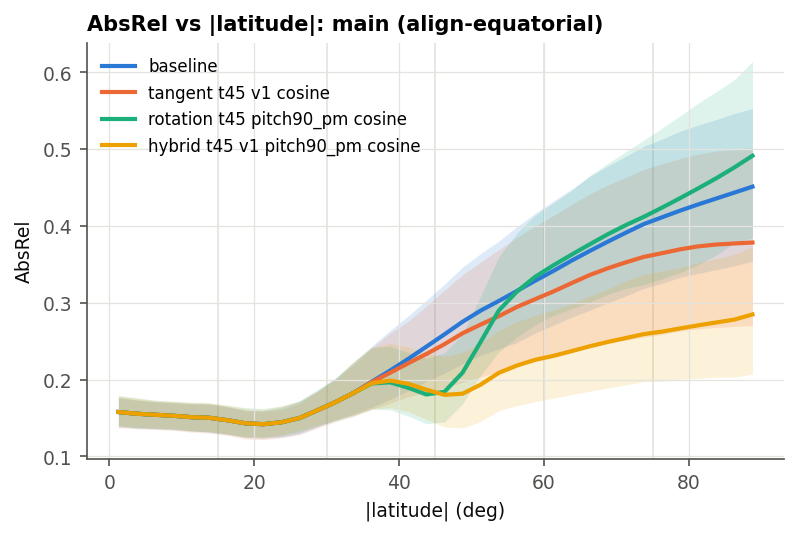
\includegraphics[width=0.94\linewidth]{core_synthetic_profile.png}
\caption{DPT-Hybrid error profile by absolute latitude on the synthetic set under equator-anchored evaluation. The profile makes visible the polar degradation and the different response of tangent, rotation, and hybrid predictions.}
\label{fig:synthetic-profile}
\end{figure}

The paired band analysis gives a more specific picture. Under equatorial alignment, the hybrid improves the $45$--$60^\circ$, $60$--$75^\circ$, and $75$--$90^\circ$ bands by 31.8\%, 34.1\%, and 36.8\%, respectively, using the ratio-of-means summary. It improved 18--20 of the 24 scenes in those bands. Under global alignment, most of the apparent benefit is absorbed into the fit; the equatorial band improves, but the polar-band change is not significant. This demonstrates why an alignment protocol is part of the research question for affine-invariant depth models, not merely an implementation detail.

The second model, MiDaS Swin2-Tiny, does not show a robust transfer of the hybrid gain under global alignment: its global AbsRel changes from 0.218 to 0.223 (not significant). Under equatorial alignment, the baseline fit is degenerate on some images, so only per-image medians are interpretable; the $75$--$90^\circ$ hybrid result is not significant. The correction therefore cannot be described as model-independent on the basis of these two models.

\subsection{External real-data check on NYC}

Table~\ref{tab:nyc} summarises the 75-image NYC run. Under global alignment, tangent inference is the safest correction: global AbsRel changes from 0.3497 to 0.3393 and polar AbsRel from 0.4265 to 0.4074. Rotation is harmful globally and in the polar region. The hybrid improves the extreme $75$--$90^\circ$ band, but its global AbsRel increases from 0.3497 to 0.3606. Under equatorial alignment, tangent and hybrid both reach 0.482 polar AbsRel from a 0.529 baseline. The size of the hybrid's synthetic gain therefore does not transfer to the real outdoor subset.

\begin{table}[t]
\caption{MiDaS DPT-Hybrid on 75 NYC street panoramas. Global and polar ($|\phi|\geq60^\circ$) AbsRel are shown for the global-fit protocol; the last column gives polar AbsRel with equatorial alignment.}
\label{tab:nyc}
\centering\small
\begin{tabular}{lrrr}
\toprule
Method & Global, \texttt{align-all} & Polar, \texttt{align-all} & Polar, \texttt{align-equatorial}\\
\midrule
Baseline & 0.3497 & 0.4265 & 0.529\\
Tangent & \textbf{0.3393} & \textbf{0.4074} & \textbf{0.482}\\
Rotation & 0.3875 & 0.4974 & 0.651\\
Hybrid & 0.3606 & 0.4132 & \textbf{0.482}\\
\bottomrule
\end{tabular}
\end{table}

\begin{figure}[t]
\centering
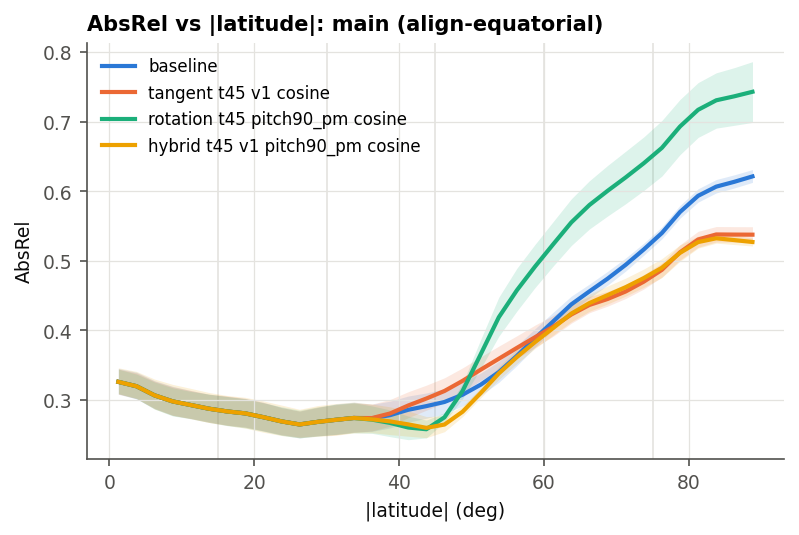
\includegraphics[width=0.94\linewidth]{core_nyc_profile.png}
\caption{DPT-Hybrid latitude profile on the NYC street panorama subset under equator-anchored evaluation. Unlike the synthetic set, the tangent and hybrid polar gains are modest and the rotation ensemble is consistently worse.}
\label{fig:nyc-profile}
\end{figure}

The domain gap matters. NYC has difficult outdoor content and far-range depth, and the equatorial error is already high. The hybrid's polar improvement under equatorial alignment is around 9\%, much smaller than the 36.8\% reduction reported for the synthetic $75$--$90^\circ$ band. Under global alignment the hybrid's overall error increases by 3.1\%. We therefore treat tangent inference, not the hybrid, as the more defensible real-data result from this comparison.

\subsection{PanoX: full-sphere 20-view inference}

Experiment 04 compares 20-view inference with the baseline and two-pole tangent method on 200 PanoX panoramas from eight environments. Table~\ref{tab:twenty-view} reports median AbsRel. Under equatorial alignment, 20-view reduces the $75$--$90^\circ$ median from 0.3468 to 0.1550; the environment-cluster bootstrap estimates a 51.77\% median gain versus baseline with a 95\% interval of [12.49\%, 54.53\%]. Under global alignment the corresponding gain is 56.81\% [25.92\%, 62.99\%]. However, the method requires 20 model calls per panorama compared with three for two-pole tangent. A subsequent direct paired audit of the same 200 scenes, resampling the eight environments, estimates a $15.55\%$ median environment gain for 20-view over two-pole tangent under align-all, but its 95\% interval is [$-84.48\%, +34.05\%$]. Under align-equatorial the estimate is $-13.37\%$ [$-69.33\%, +18.00\%$]. Both intervals include zero, and the point-estimate ordering changes with the alignment protocol. Thus the PanoX results establish improvement over baseline for both corrections, but do not establish that the more expensive 20-view method is better than two-pole tangent. The intervals are broad because only eight environment clusters are available.

\begin{table}[t]
\caption{Experiment 04: median AbsRel on 200 PanoX panoramas. Calls denote model forward passes per image.}
\label{tab:twenty-view}
\centering\small
\begin{tabular}{llrrrr}
\toprule
Protocol & Method & All & $60$--$75^\circ$ & $75$--$90^\circ$ & Calls\\
\midrule
\texttt{align-all} & Baseline & 0.1898 & 0.1394 & 0.1514 & 1\\
 & Two-pole tangent & 0.1632 & 0.1020 & 0.0950 & 3\\
 & 20-view & 0.1645 & \textbf{0.0801} & \textbf{0.0832} & 20\\
\midrule
\texttt{align-equatorial} & Baseline & 0.2321 & 0.2389 & 0.3468 & 1\\
 & Two-pole tangent & 0.1913 & 0.1661 & 0.1659 & 3\\
 & 20-view & \textbf{0.1615} & \textbf{0.1429} & \textbf{0.1550} & 20\\
\bottomrule
\end{tabular}
\end{table}

\begin{figure}[t]
\centering
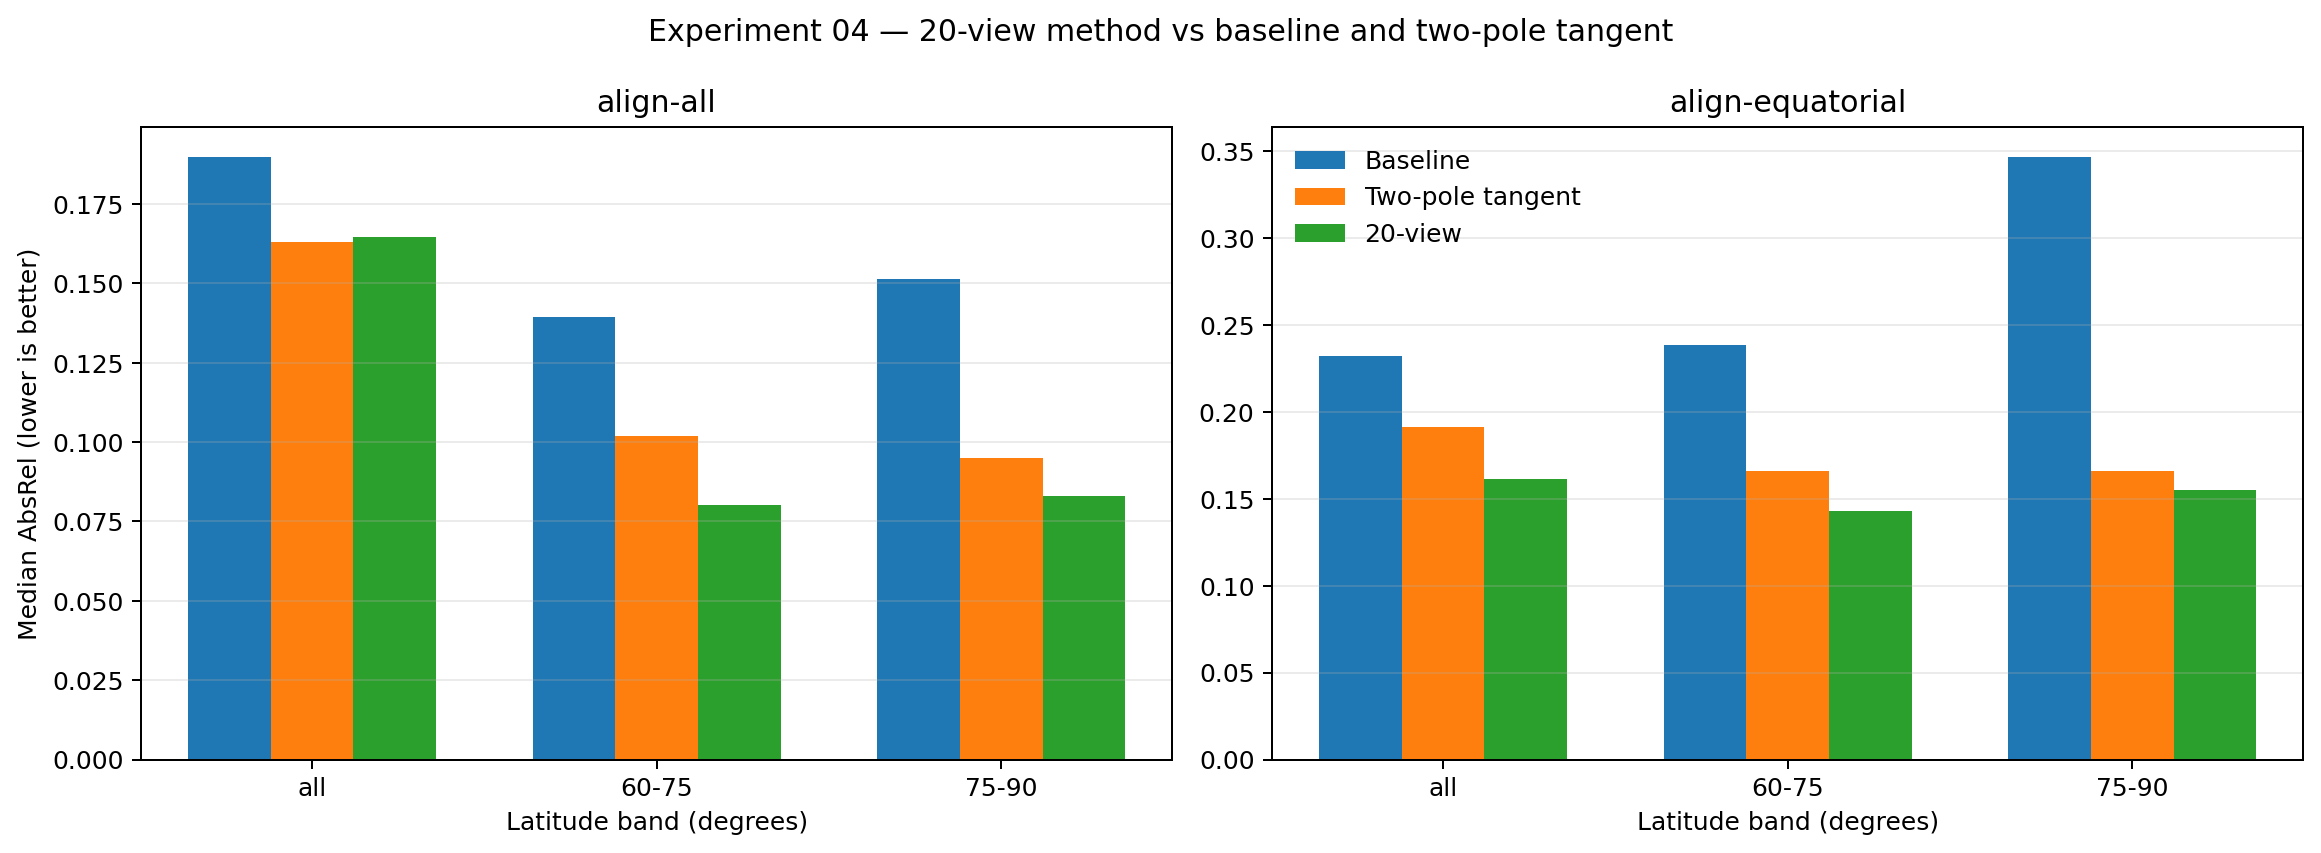
\includegraphics[width=0.94\linewidth]{exp04_20view_comparison.png}
\caption{Experiment 04 comparison of baseline, two-pole tangent, and 20-view inference across latitude bands under both alignment protocols.}
\label{fig:twenty-view}
\end{figure}

\subsection{PanoX: field of view matters more than resolution}

Experiment 05 evaluates 12 FOV--resolution combinations on the same 200 PanoX panoramas. Table~\ref{tab:fov} fixes tangent resolution at $512^2$ to isolate the FOV trend. Moving from $70^\circ$ to $110^\circ$ or $130^\circ$ substantially lowers polar median AbsRel. The best raw value depends on the alignment protocol: $130^\circ$ gives 0.0915 under \texttt{align-all}, while $110^\circ$ gives 0.1644 under \texttt{align-equatorial}. The paired cluster bootstrap confirms that each of the $90^\circ$--$130^\circ$ settings improves over baseline in the $75$--$90^\circ$ band, but it does not rank those FOVs against one another. Curves across $256^2$, $384^2$, and $512^2$ are close at each FOV, suggesting diminishing returns from increasing resolution in this range.

\begin{table}[t]
\caption{Experiment 05: median AbsRel in the $75$--$90^\circ$ band for $512\times512$ tangent views on 200 PanoX panoramas.}
\label{tab:fov}
\centering\small
\begin{tabular}{rrr}
\toprule
FOV & \texttt{align-all} & \texttt{align-equatorial}\\
\midrule
$70^\circ$ & 0.1400 & 0.3269\\
$90^\circ$ & 0.1092 & 0.1807\\
$110^\circ$ & 0.0949 & \textbf{0.1644}\\
$130^\circ$ & \textbf{0.0915} & 0.1702\\
\bottomrule
\end{tabular}
\end{table}

\begin{figure}[t]
\centering
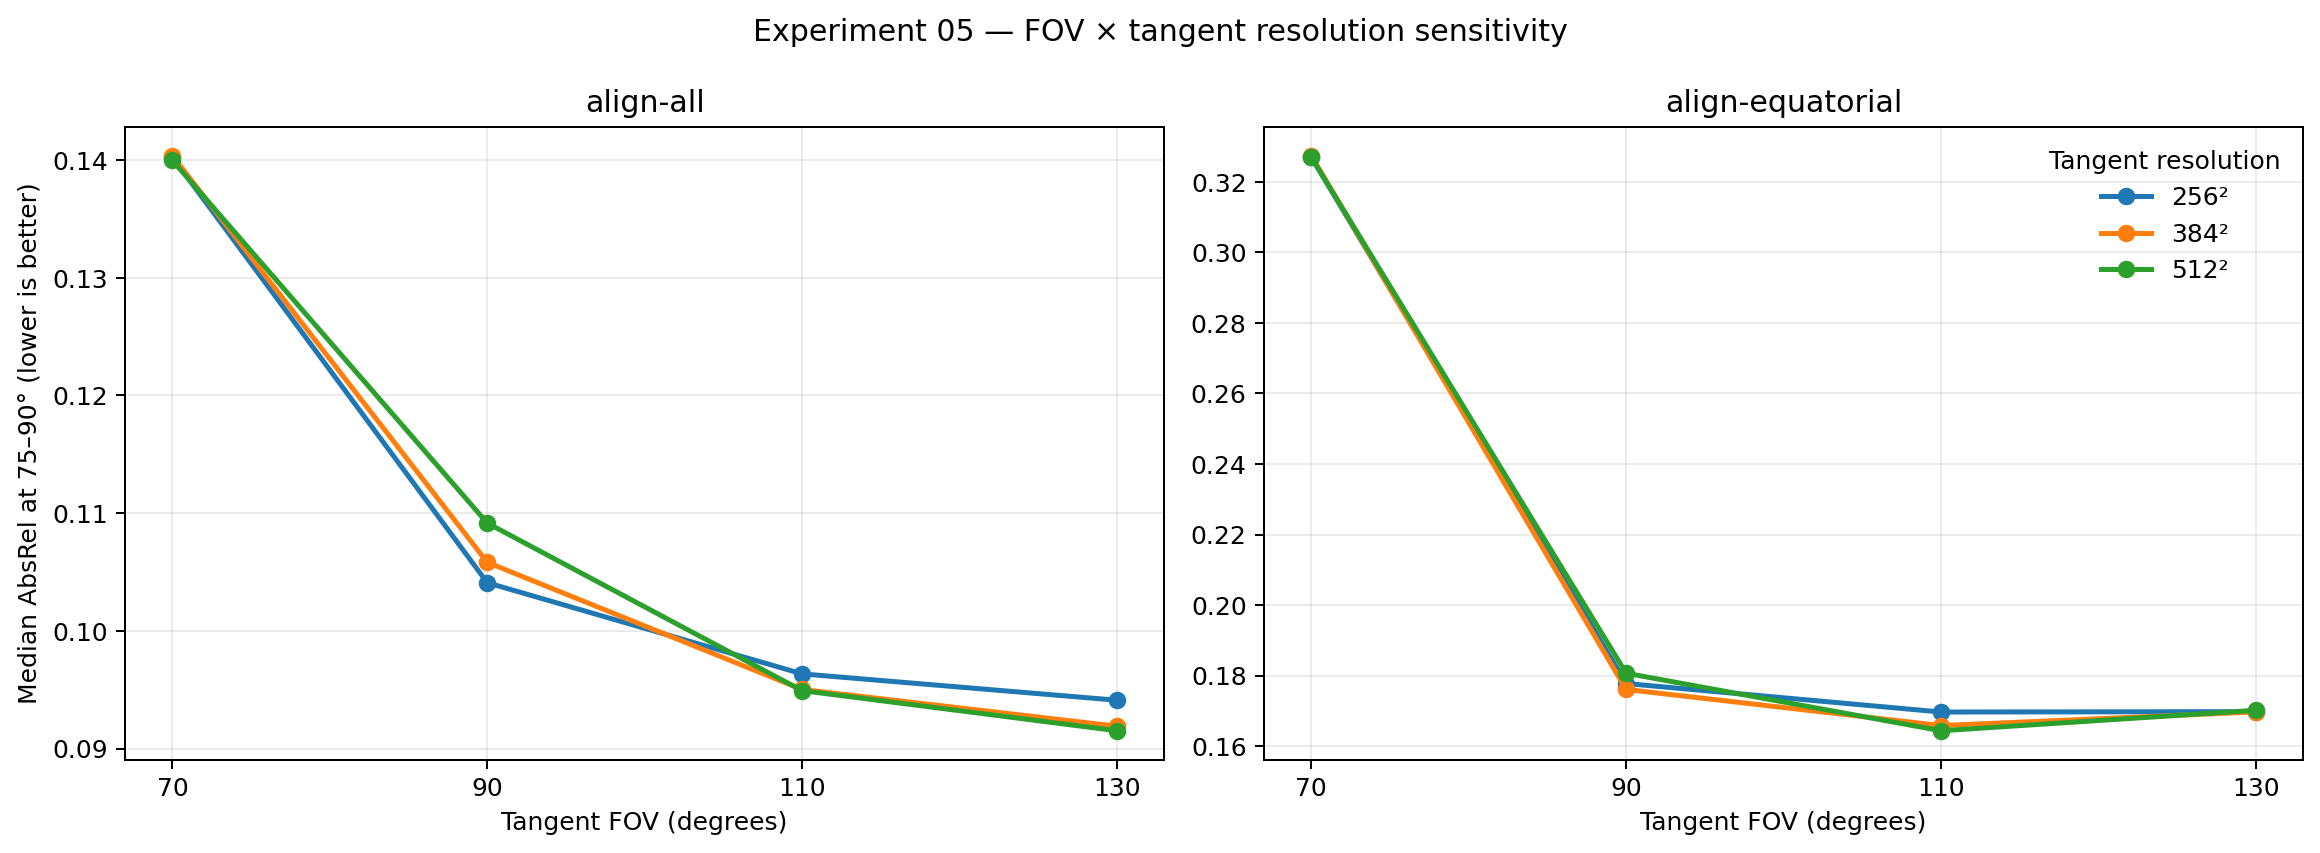
\includegraphics[width=0.94\linewidth]{exp05_fov_resolution_sweep.png}
\caption{Experiment 05: polar median AbsRel as a function of tangent FOV and resolution. Wider FOVs improve substantially over $70^\circ$; resolution has a smaller effect in the tested range.}
\label{fig:fov}
\end{figure}

\subsection{DA360: alignment protocol and environment transfer}

Experiment 01 uses 200 Structured3D scenes to compare scale-only and affine disparity alignment for DA360. Since DA360 is specified as scale-invariant disparity, scale-only is the principled primary protocol. Under \texttt{align-all}, the $75$--$90^\circ$ median AbsRel is 0.0056 for scale-only and 0.0054 for affine; the paired gain is $-0.45\%$ with a 95\% interval of [$-6.27\%$, $+1.85\%$]. Under \texttt{align-equatorial}, values are 0.0070 and 0.0095, and the scale-only gain is $+5.74\%$ [$+0.27\%$, $+17.95\%$]. This is evidence that the evaluation fit changes the comparison; it is not evidence that scale-only uniformly lowers prediction error.

\begin{figure}[t]
\centering
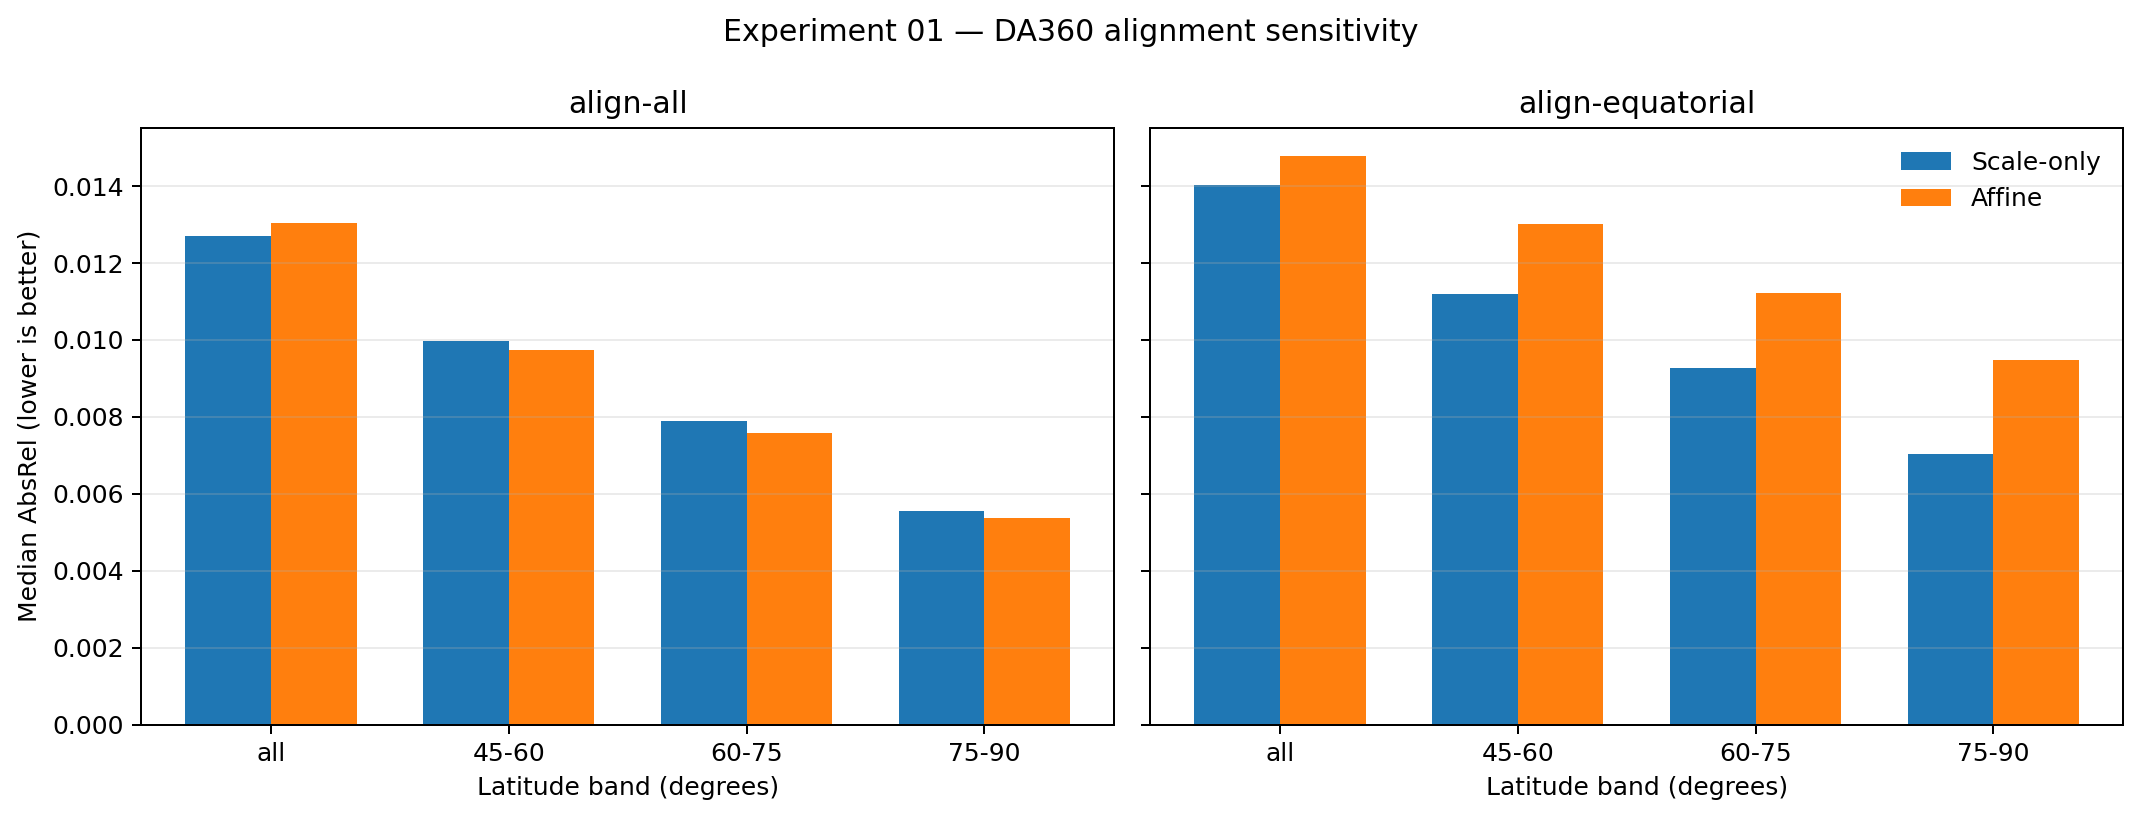
\includegraphics[width=0.94\linewidth]{exp01_scale_vs_affine.png}
\caption{Experiment 01: DA360 scale-only and affine median AbsRel by latitude band under both alignment protocols.}
\label{fig:scale-affine}
\end{figure}

Experiment 02 asks whether a rotation threshold selected on other PanoX environments transfers to a held-out environment. All eight LOEO folds select the baseline/no-correction option under the 0.50\% minimum calibration-gain rule. The resulting mean AbsRel is 0.0389 (median 0.0282). A fixed $45^\circ$ gate has mean AbsRel 0.0877 and a median relative gain of $-55.44\%$ versus baseline; even the per-environment oracle is worse in aggregate (mean 0.0720). The result is a negative finding for this latitude/environment-conditioned gate: abstention is safer than applying a threshold that fails to transfer. It does not rule out image-conditioned gates based on visual structure, which remain untested in Experiment 06.

\subsection{Student distillation prototype}

The saved Experiment 03 evaluation covers 50 scenes from the held-out ClothingStore and ModularBakeryShop environments. Under \texttt{align-all}, teacher/student median AbsRel is 0.0637/0.3130 globally, 0.0270/0.2837 at $60$--$75^\circ$, and 0.0130/0.3136 at $75$--$90^\circ$. Under equatorial alignment the student remains much worse (global 0.8123 and polar values 1.1819 and 1.3171). The prototype therefore did not preserve the teacher's depth quality on these held-out scenes.

This finding has a reproducibility caveat: the evaluation summary references a Kaggle checkpoint path, but the corresponding `best.pt` file and training log are not present in the local checkout. The evaluation report and per-scene CSV are retained; full reproduction requires restoring the student checkpoint and training record.

\section{Discussion}

Three lessons emerge. First, alignment protocol is a first-order variable for relative-depth evaluation. The synthetic hybrid appears strongly beneficial when the equator anchors scale, but the standard global fit shows little polar improvement and a much smaller global gain. A paper that reports only one fit risks overstating or understating the effect. Second, geometric coverage matters: on PanoX, 20-view inference and wider FOVs improve polar medians, but the 20-view method spends substantially more inference compute, and the current statistics do not demonstrate a pairwise win over two-pole tangent. Third, these results are domain- and model-dependent. The hybrid's synthetic advantage shrinks on NYC; the DA360 LOEO gate abstains in all folds; and the student prototype is much worse than its teacher.

The practical choice is therefore not a single universally best correction. For the tested MiDaS/NYC setting, tangent views are a conservative improvement. For the PanoX experiment, 20-view inference gives the best reported polar median among the compared methods but at a large call-count penalty. For the FOV sweep, values above $70^\circ$ are preferable in the tested range, but no alignment-independent optimum is established. For DA360, scale-only should be the headline fit on semantic grounds, while both fits should remain visible as a sensitivity analysis.

\section{Limitations and evidence boundaries}

The synthetic core study has only 24 procedurally generated scenes; its geometry and texture are simpler than real captures. The NYC comparison has 75 panoramas from one outdoor domain and should not be interpreted as broad cross-domain validation. PanoX follow-ups contain 200 panoramas but only eight independent environment clusters; cluster-level intervals are more appropriate than treating adjacent panoramas as independent. The paired bootstrap in Experiments 04 and 05 compares each method with baseline and does not establish pairwise significance between alternatives.

The student result is not fully reproducible from this checkout because its checkpoint is missing. Experiment 06 is code/design only and has no result. The Holo360D indoor loader smoke test used 60 frames from training scenes and is not a held-out benchmark; no Holo360D test-split result is included here. Although the repository contains a DAP wrapper/configuration, these Lokesh results do not evaluate the DAP model. The NYC data source is the DAP dataset, but the network used in that experiment is MiDaS DPT-Hybrid. No claim about DAP's accuracy or about held-out Holo360D performance is made.

Finally, the experiments are not one homogeneous benchmark: the core synthetic/NYC runs, DA360 alignment study, PanoX gate, 20-view/FOV studies, and student evaluation differ in backbone, dataset, sample unit, and alignment protocol. We retain this separation in the report and do not combine their raw metric values into a single leaderboard.

\section{Conclusion}

Inference-time projection changes can improve polar depth estimates, but their value is conditional. On synthetic MiDaS evaluation, the hybrid is strong under equatorial alignment but its polar advantage largely disappears under global affine alignment. On NYC, tangent views are more reliable than rotation or hybrid inference. On PanoX, wider FOVs and full-sphere 20-view coverage improve polar median error, with the latter requiring 20 model calls per image. DA360's scale protocol and threshold-transfer experiments further show that alignment and domain transfer need to be tested directly; the student prototype supplies a negative transfer result. The main conclusion is not that one projection wins, but that view geometry, scale anchoring, dataset domain, and compute must be evaluated together.

\section*{Reproducibility and artifact map}

The source artifacts are retained in the \texttt{Lokesh/} project folder. Core results are stored under \url{results/midas_dpt_hybrid_synthetic/}, \url{results/midas_swin2_tiny_synthetic/}, and \url{results/midas_dpt_hybrid_nyc/}. Selected follow-up runs are identified by their timestamps in \url{followup_experiments/RESULTS.md}. Every selected run keeps a human-readable report and a machine-readable summary; per-scene CSVs are available for Studies 01, 02, 04, and 05. The report source, NeurIPS style file, and figures are stored together in \url{Report/draft/}.

\begin{thebibliography}{9}
\small
\bibitem{ranftl2021dpt} R. Ranftl, A. Bochkovskiy, and V. Koltun. Vision Transformers for Dense Prediction. In \emph{Proceedings of the IEEE/CVF International Conference on Computer Vision (ICCV)}, 2021.
\bibitem{rey2022} M. Rey-Area, M. Yuan, and C. Richardt. 360MonoDepth: High-resolution 360$^\circ$ monocular depth estimation. In \emph{Proceedings of the IEEE/CVF Conference on Computer Vision and Pattern Recognition (CVPR)}, 2022. arXiv:2111.15669.
\bibitem{wang2024} N.-H. Wang and Y.-L. Liu. Depth Anywhere: Enhancing 360 monocular depth estimation via perspective distillation and unlabeled data augmentation. 2024. arXiv:2406.12849.
\bibitem{cao2024panda} Z. Cao, J. Zhu, W. Zhang, H. Ai, H. Bai, H. Zhao, and L. Wang. PanDA: Towards panoramic depth anything with unlabeled panoramas and M\"obius spatial augmentation. 2024. arXiv:2406.13378.
\bibitem{guo2025dac} Y. Guo, S. Garg, S. M. H. Miangoleh, X. Huang, and L. Ren. Depth Any Camera: Zero-shot metric depth estimation from any camera. 2025. arXiv:2501.02464.
\bibitem{lin2025dap} X. Lin, M. Song, D. Zhang, W. Lu, H. Li, B. Du, M.-H. Yang, T. Nguyen, and L. Qi. Depth Any Panoramas: A foundation model for panoramic depth estimation. 2025. arXiv:2512.16913.
\bibitem{jiang2025da360} H. Jiang, Z. Song, Z. Lou, R. Xu, and M. Tan. Depth Anything in 360$^\circ$: Towards scale invariance in the wild. 2025. arXiv:2512.22819.
\end{thebibliography}

\end{document}